\documentclass[10pt,a4paper]{IEEEtran}
\usepackage[latin1]{inputenc}
\usepackage{amsmath}
\usepackage{amsfonts}
\usepackage{amssymb}
\usepackage{graphicx}
\usepackage{float}
\usepackage{gensymb}
\usepackage{hyperref}
\usepackage{cite}
\usepackage[justification=centering, font={small,it}]{caption}
\author{Dicson Wijaya (1002289), Wenkie Lau (1002219), \\ Mok Jun Neng (1002219), Charlotte Phang (1002277),\\ Martin Tan (1002173)}
\title{Physical World 2D Report}
\begin{document}
	\maketitle
	\section{Finding $\lambda_{algae bottle}$}
	Based on the Fourier's law of thermal conduction: $R = \frac{\Delta T}{\dot{Q}}$, and using the substitutions $\dot{Q} = mc \dot{T} = \rho V c \dot{T}$, where $\rho$, $V$ and $c$ is the density, volume and specific heat capacity of water respectively. we can write a first order differential equation:
		
	$$\Delta T = T - T_{amb} = -R \rho V c \frac{dT}{dt}$$
	Solving this differential equation,
	$$\int_{0}^{t} dt = -R \rho V c \int_{T_{initial}}^{T}\frac{1}{T-T_{amb}} dT$$
	$$\frac{t}{R \rho V c} = \ln \left| \frac{T - T_{amb}}{T_i - T_{amb}} \right|$$
	$$\left( T_{initial} - T_{amb} \right) \exp(-\frac{t}{R \rho V c}) = T - T_{amb}$$
	$$\Delta T = \Delta T_{initial} \cdot \exp(-\frac{t}{R \rho V c})$$
	
	It can be concluded that a best fit exponential curve of a $\Delta T$ against $t$ plot may be used to empirically determine the value of $\lambda_{algae bottle}$.
	\section{Methodology}
	Figure \ref{fig:methodology} shows the experimental set up for determining $\lambda_{algae bottle}$.
	
 	\begin{figure}[H]
 		\begin{center}
 			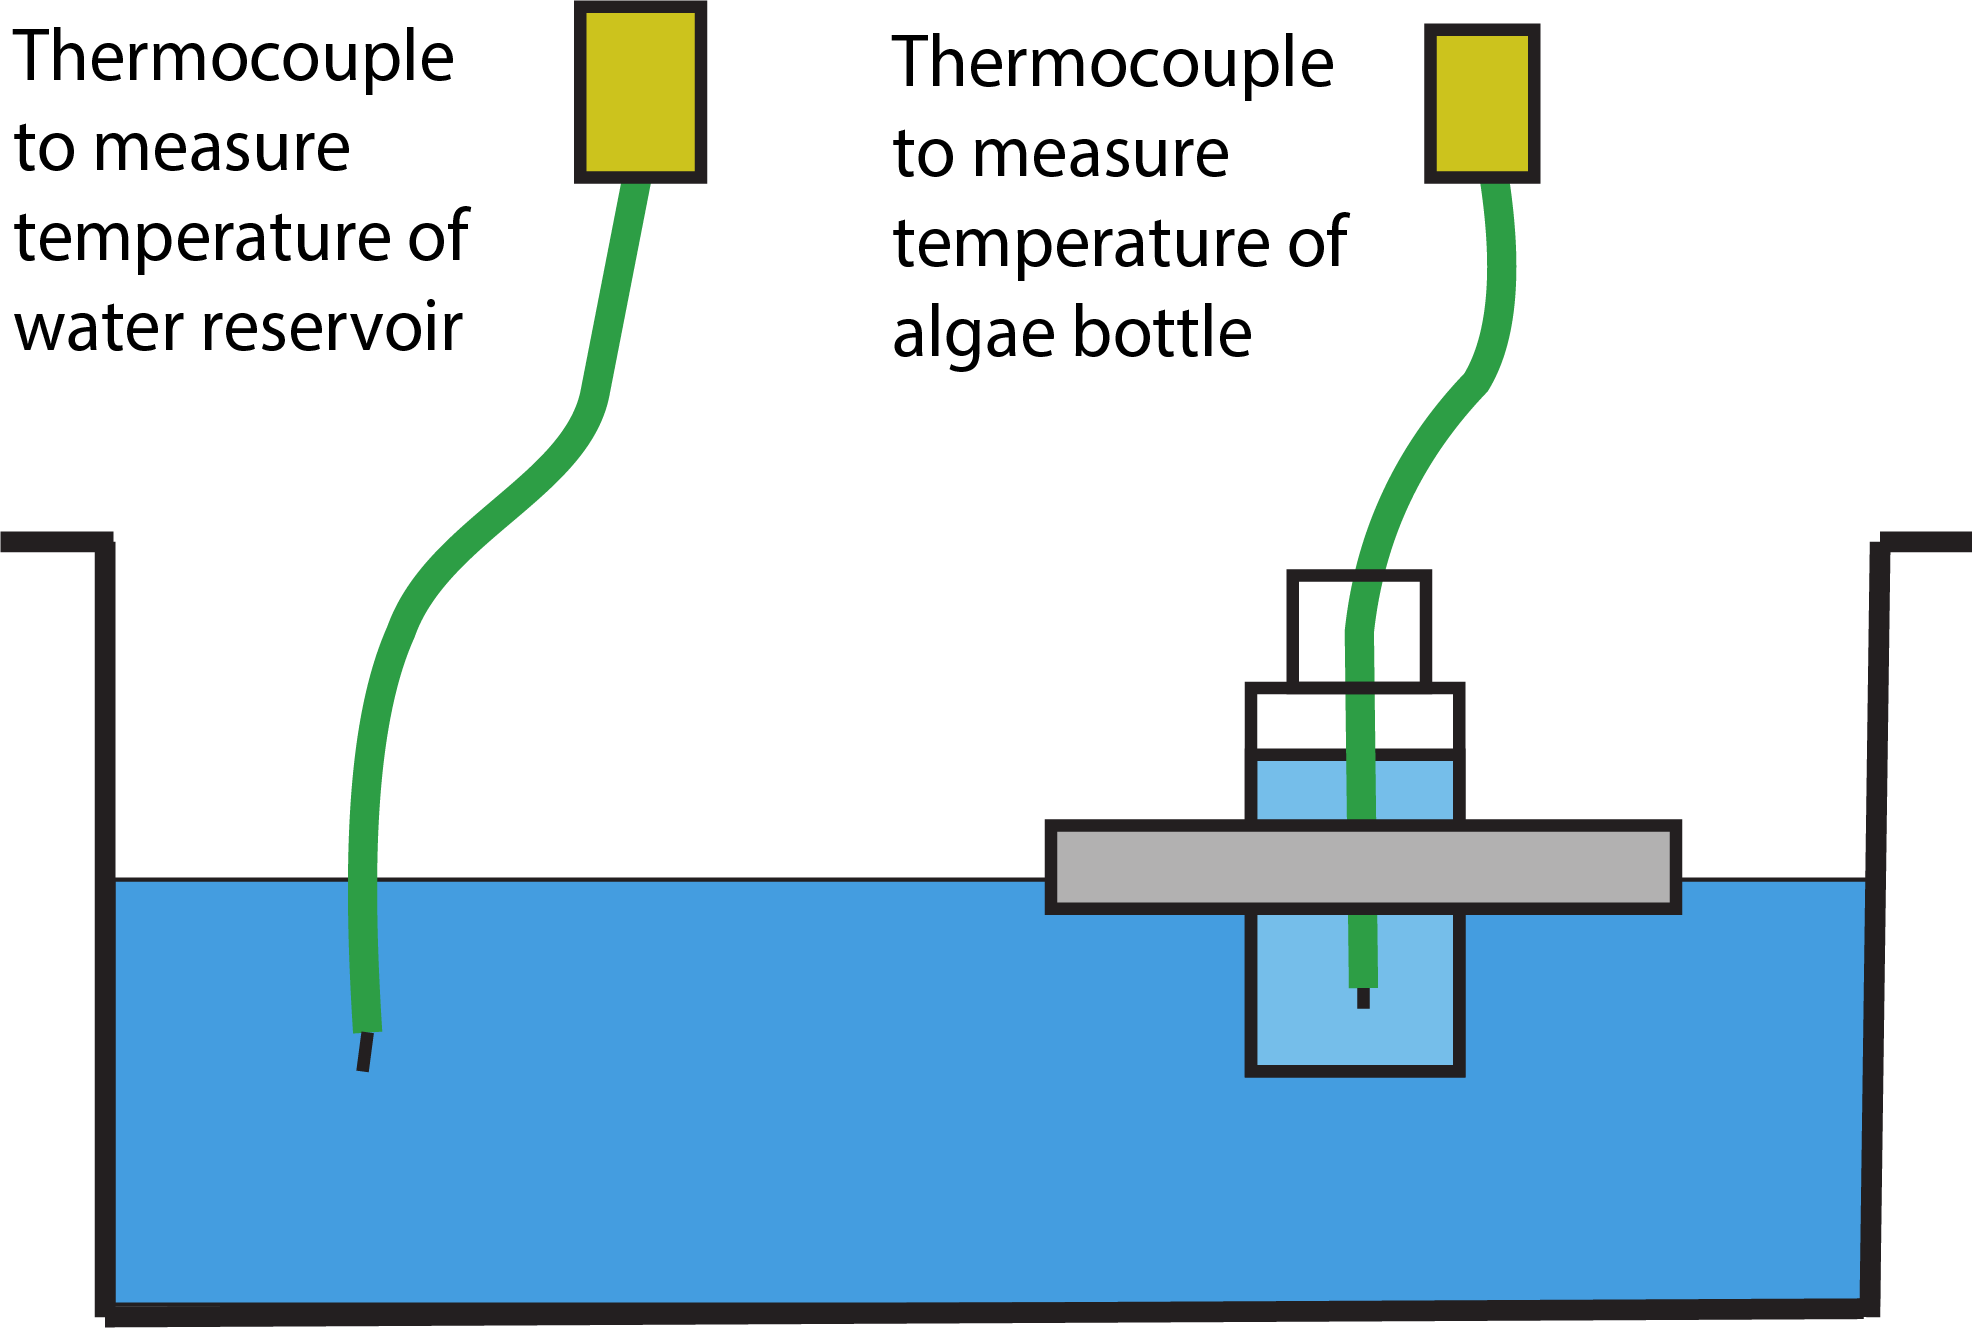
\includegraphics[width=0.5\textwidth]{methodology.png}
 			\caption{Experimental set up}
 			\label{fig:methodology}
 		\end{center}
 	\end{figure} 
	
	The following methodology was used to obtain data:
	\begin{enumerate}
		\item Fill the bottle with 30ml of hot water.
		\item Place thermocouples in the bottle and the tank as shown in Figure \ref{fig:methodology}.
		\item Use a video camera to record the displays of the digital thermometer and a stopwatch.
		\item Place the (bottle with floatation device) into the water resevoir and as shown in Figure \ref{fig:methodology} and start the stopwatch.
		\item Record for more than 100 seconds.
		\item Review the footage and record the time displayed by the stopwatch at every temperature decrement ($0.1 \degree C$).
	\end{enumerate}
	
	After obtaining data to calculate $\lambda_{algae bottle}$, another experiment was carried out to determine $\lambda_{tubing}$. Silicone tubing was stuffed into the container, and the cooling curve data was also obtained by the same method as the previous experiment.
	
	\section{Data Analysis}
	Once the data was obtained, a best fit exponential curve in the form $y = Ae^{-Bx}$, where $A, B \in \mathbb{R^{+}}$, was plotted in Microsoft Excel. (See figure \ref{fig:graph_lambdaBottle})
	
	\begin{figure}[H]
		\begin{center}
			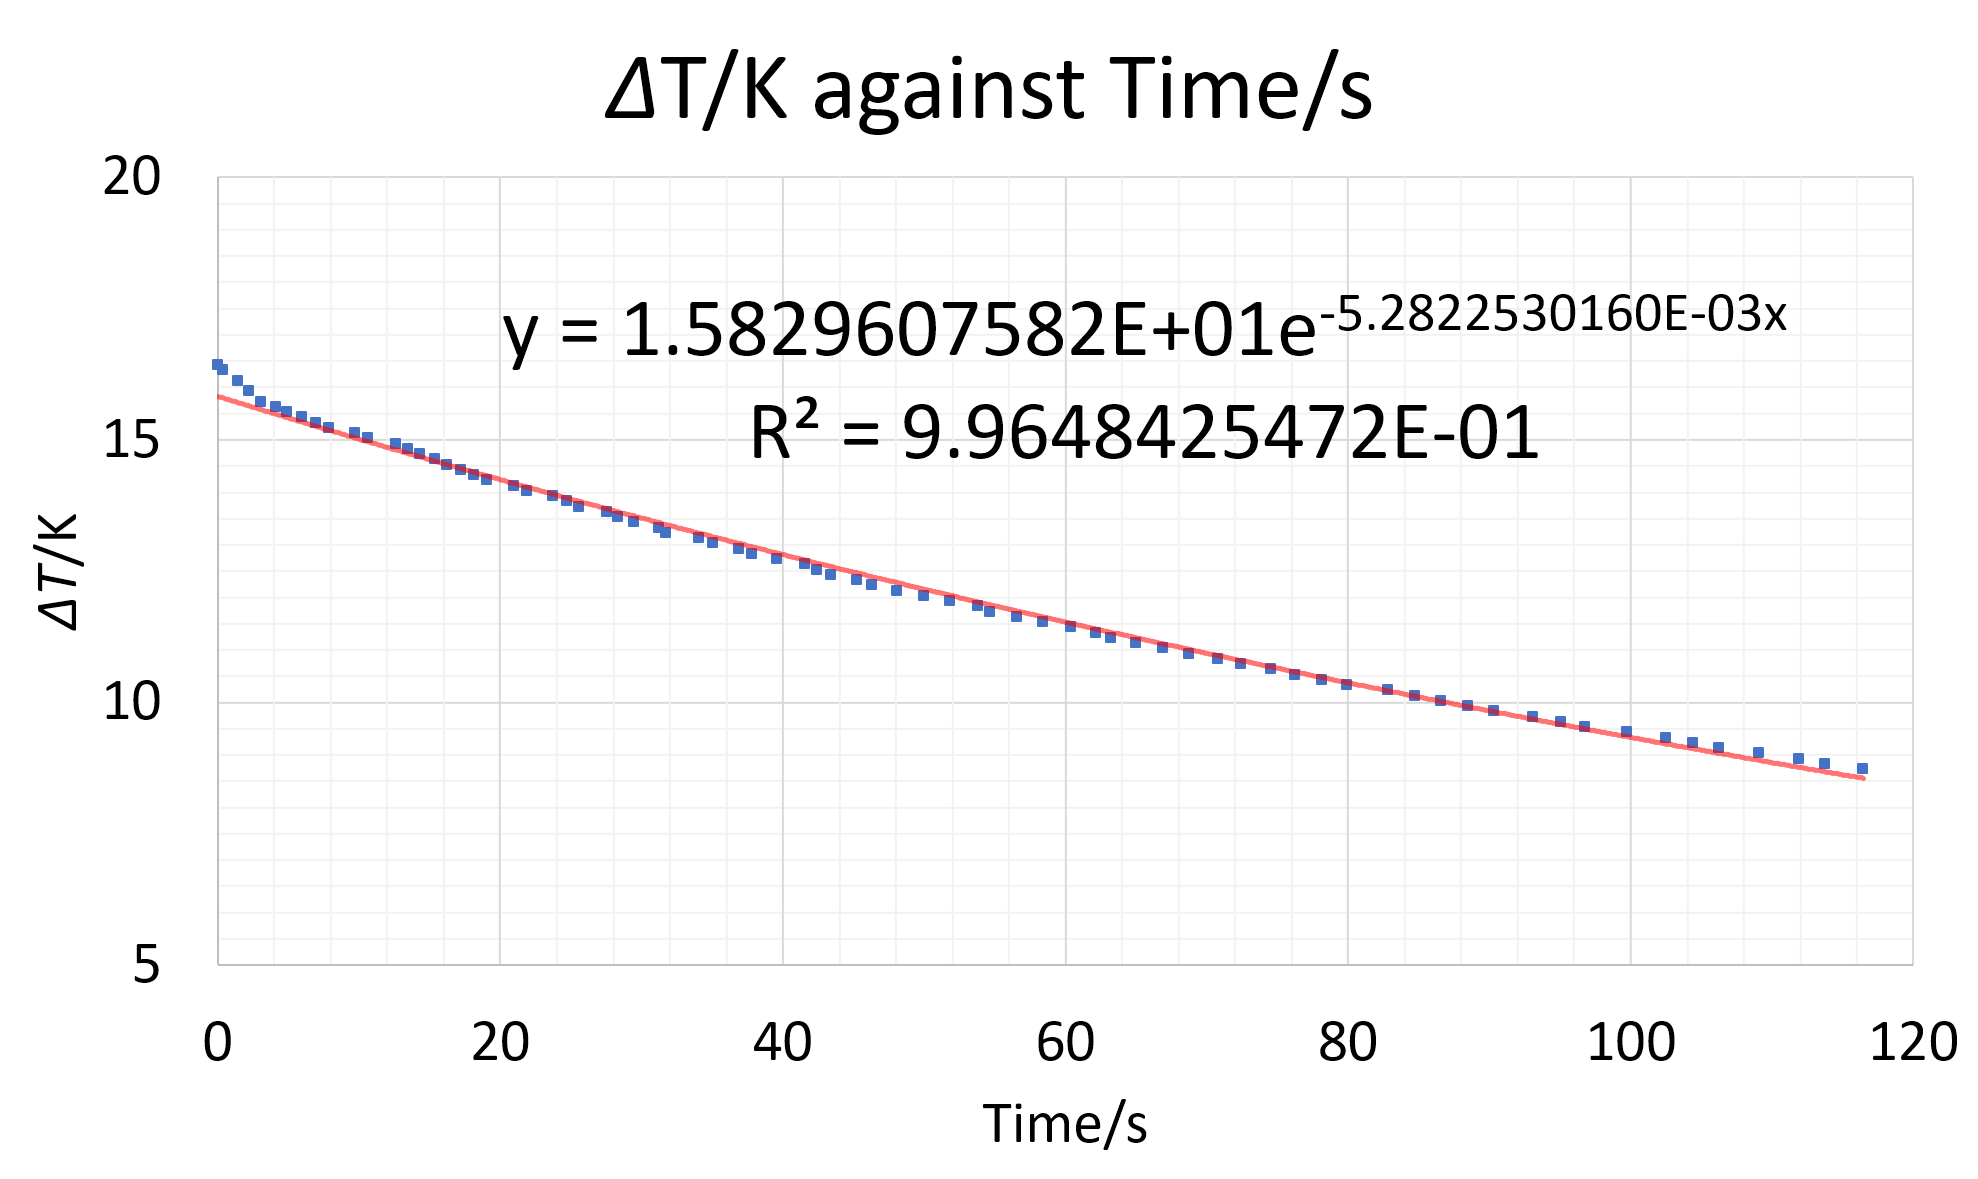
\includegraphics[width=0.5\textwidth]{graph_lambdaBottle.png}
			\caption{Graph of $\Delta T/K$ across bottle wall against Time/s}
			\label{fig:graph_lambdaBottle}
		\end{center}
	\end{figure} 
	
	The best fit curve was found to be: 
	$$y = 1.58296 \times 10^{1} \cdot \exp(-5.28225\times 10^{-3}\cdot t)$$
	
	Given $B = 5.28225\times 10^{-3}$, we can empirically find $R$ by:
	$$R_{algae bottle} = \frac{1}{\lambda_{algae bottle}} = \frac{1}{B \rho V c}$$
	
	Given $\rho = 0.9881 g \cdot cm^{-3}$ at $50 \degree C$ (see reference \cite{waterDensity}), $c = 4.18 J g^{-1} K^{-1}$ (see reference \cite{waterHeatCap}), and $V = 30 cm^{-3}$ (measured), then we can determine using the same methods of data analysis:
	$$\lambda_{algae bottle} = 0.654512033 W K^{-1}$$
	$$\lambda_{tubing} = 0.360332327W K^{-1}$$
	
	Using the value of $\lambda_{algae bottle}$ and the dimensions of the algae bottle, we are able to find the thermal conductivity $k$ of the polystyrene \cite{polystyreneBottle} algae bottle.
	$$k_{polystyrene} = 1.7651032 \times 10^{-1} W m^{-1} K^{-1}$$
	Based on online sources \cite{polystyreneConductivity}, the conductivity of polystyrene (non-expanded HIPS) is approximately $1.72 \times 10^{-1} W m^{-1} K^{-1}$, indicating that the result attained is accurate.
	
	
 	\section{Design of Heat Exchanger}
 	Since the calculated value of $\lambda_{algae bottle}$ is 82\% higher than the calculated $\lambda_{tubing}$, a heat exchanger was designed to exploit this higher heat conductance to remove heat more rapidly from the bottle. This allows for a larger heat load (such as from the sun) to be placed on the algae bottle, both increasing the safety margin of acceptable heat load before actuator saturation (i.e. peristaltic pump running at full power) and also energy efficiency at a constant heat load.\\
 	
 	A ``water jacket'' design was created in Fusion360 Computer Aided Design (CAD) software and subsequently 3D printed. Figure \ref{fig:heat_exchanger_side} below is rendered in a transparent material to show the internal structure of the heat exchanger. The inlet is situated at the bottom to allow the pump to fill the container fully; this will also allow the colder water to remain at the bottom while hotter water rises to the top of the heat exchanger and then expelled from the outlet.
 		\begin{figure}[H]
 			\begin{center}
 				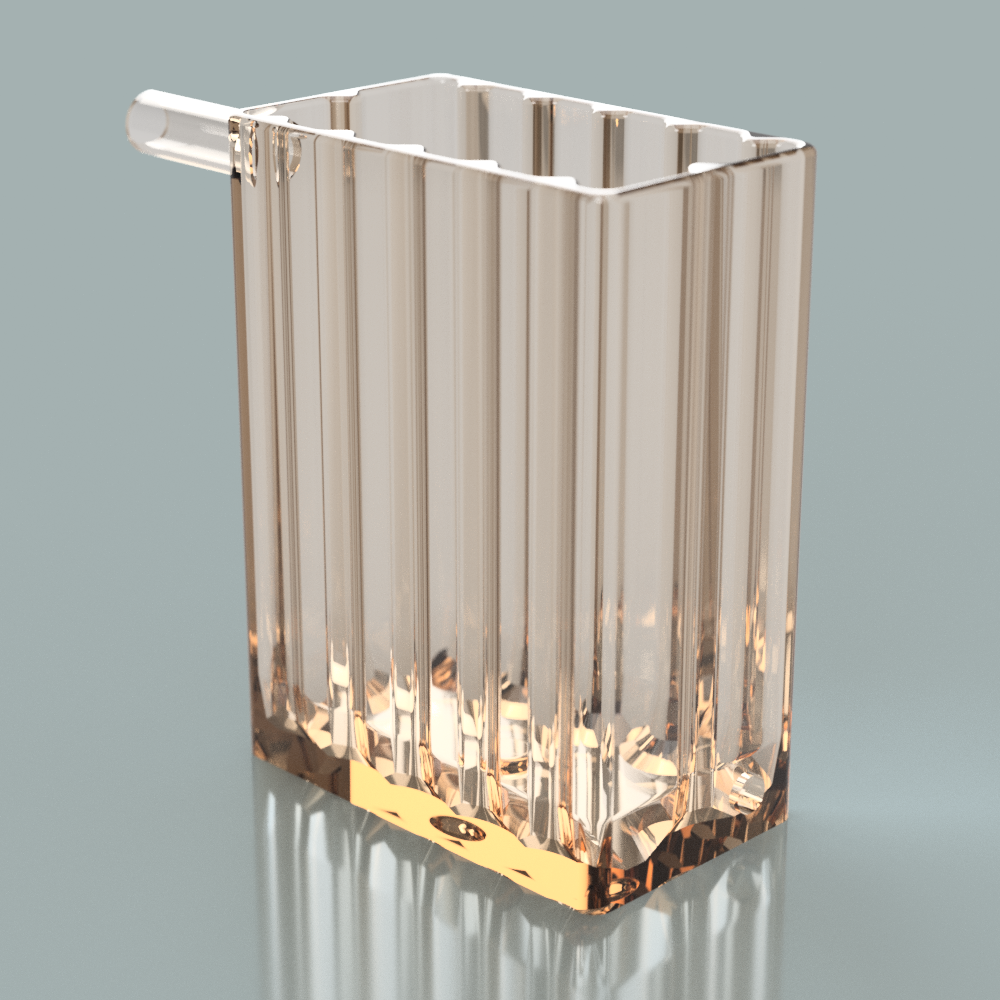
\includegraphics[width=0.3\textwidth]{heat_exchanger_side.png}
 				\caption{Internal Structure of the Heat Exchanger}
 				\label{fig:heat_exchanger_side}
 			\end{center}
 		\end{figure}
 	
 	Figure \ref{fig:heat_exchanger_top} below clearly shows the triangular protrusions on the inner wall of the heat exchanger which creates channels for the cooling water to flow around the algae bottle while minimising contact area.
 	
 		\begin{figure}[H]
 			\begin{center}
 				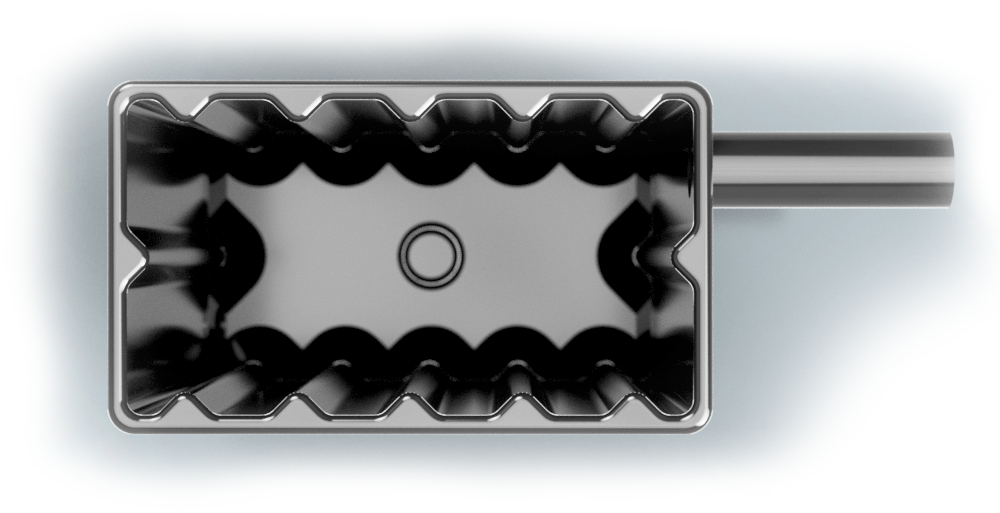
\includegraphics[width=0.3\textwidth]{heat_exchanger_top.png}
 				\caption{Top View of the Heat Exchanger}
 				\label{fig:heat_exchanger_top}
 			\end{center}
 		\end{figure}
 	Figure \ref{fig:air_gaps} below shows air gaps in the wall of an incompletely 3D printed heat exchanger which minimises heat gain or heat loss to the surroundings when the pump is not active so as to maintain temperature small temperature range for a long period.
 		\begin{figure}[H]
 			\begin{center}
 				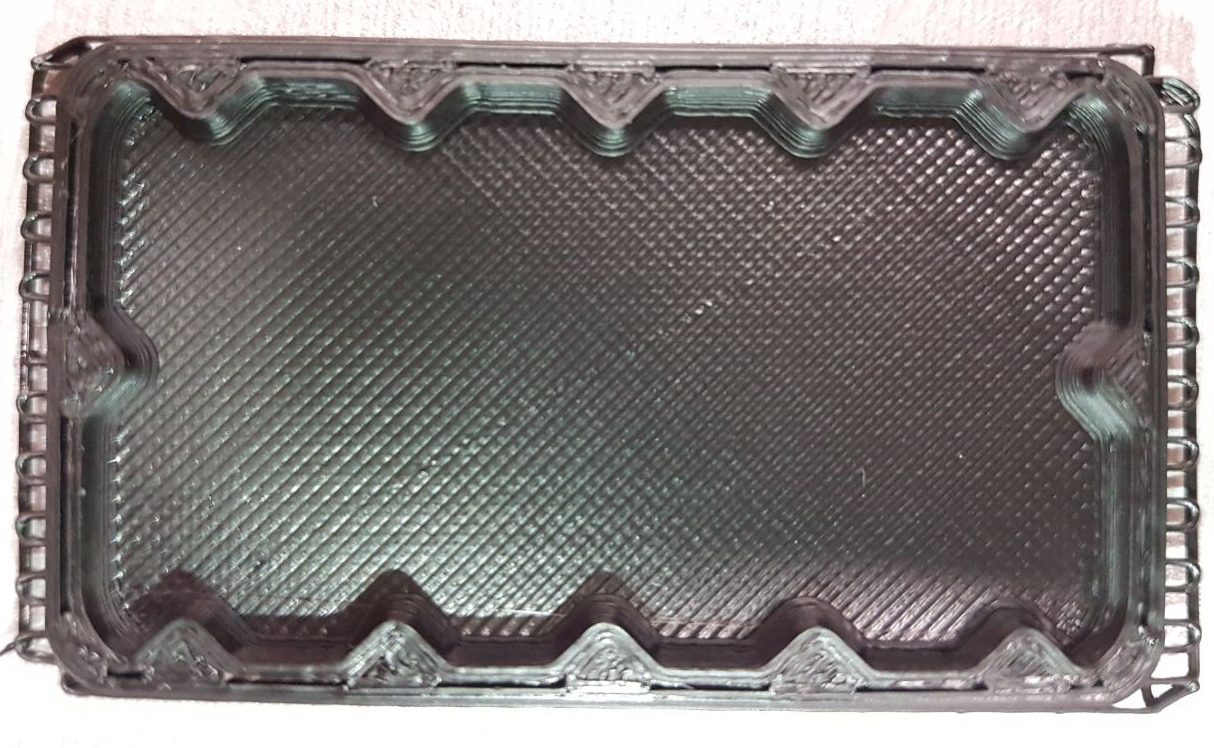
\includegraphics[width=0.35\textwidth]{air_gaps.jpeg}
 				\caption{Incomplete 3D printed heat exchanger showing air gaps}
 				\label{fig:air_gaps}
 			\end{center}
 		\end{figure}
 	Figure \ref{fig:actual_heatExchanger} below shows the actual 3D printed heat exchanger with an algae bottle fitted.
 		\begin{figure}[H]
 			\begin{center}
 				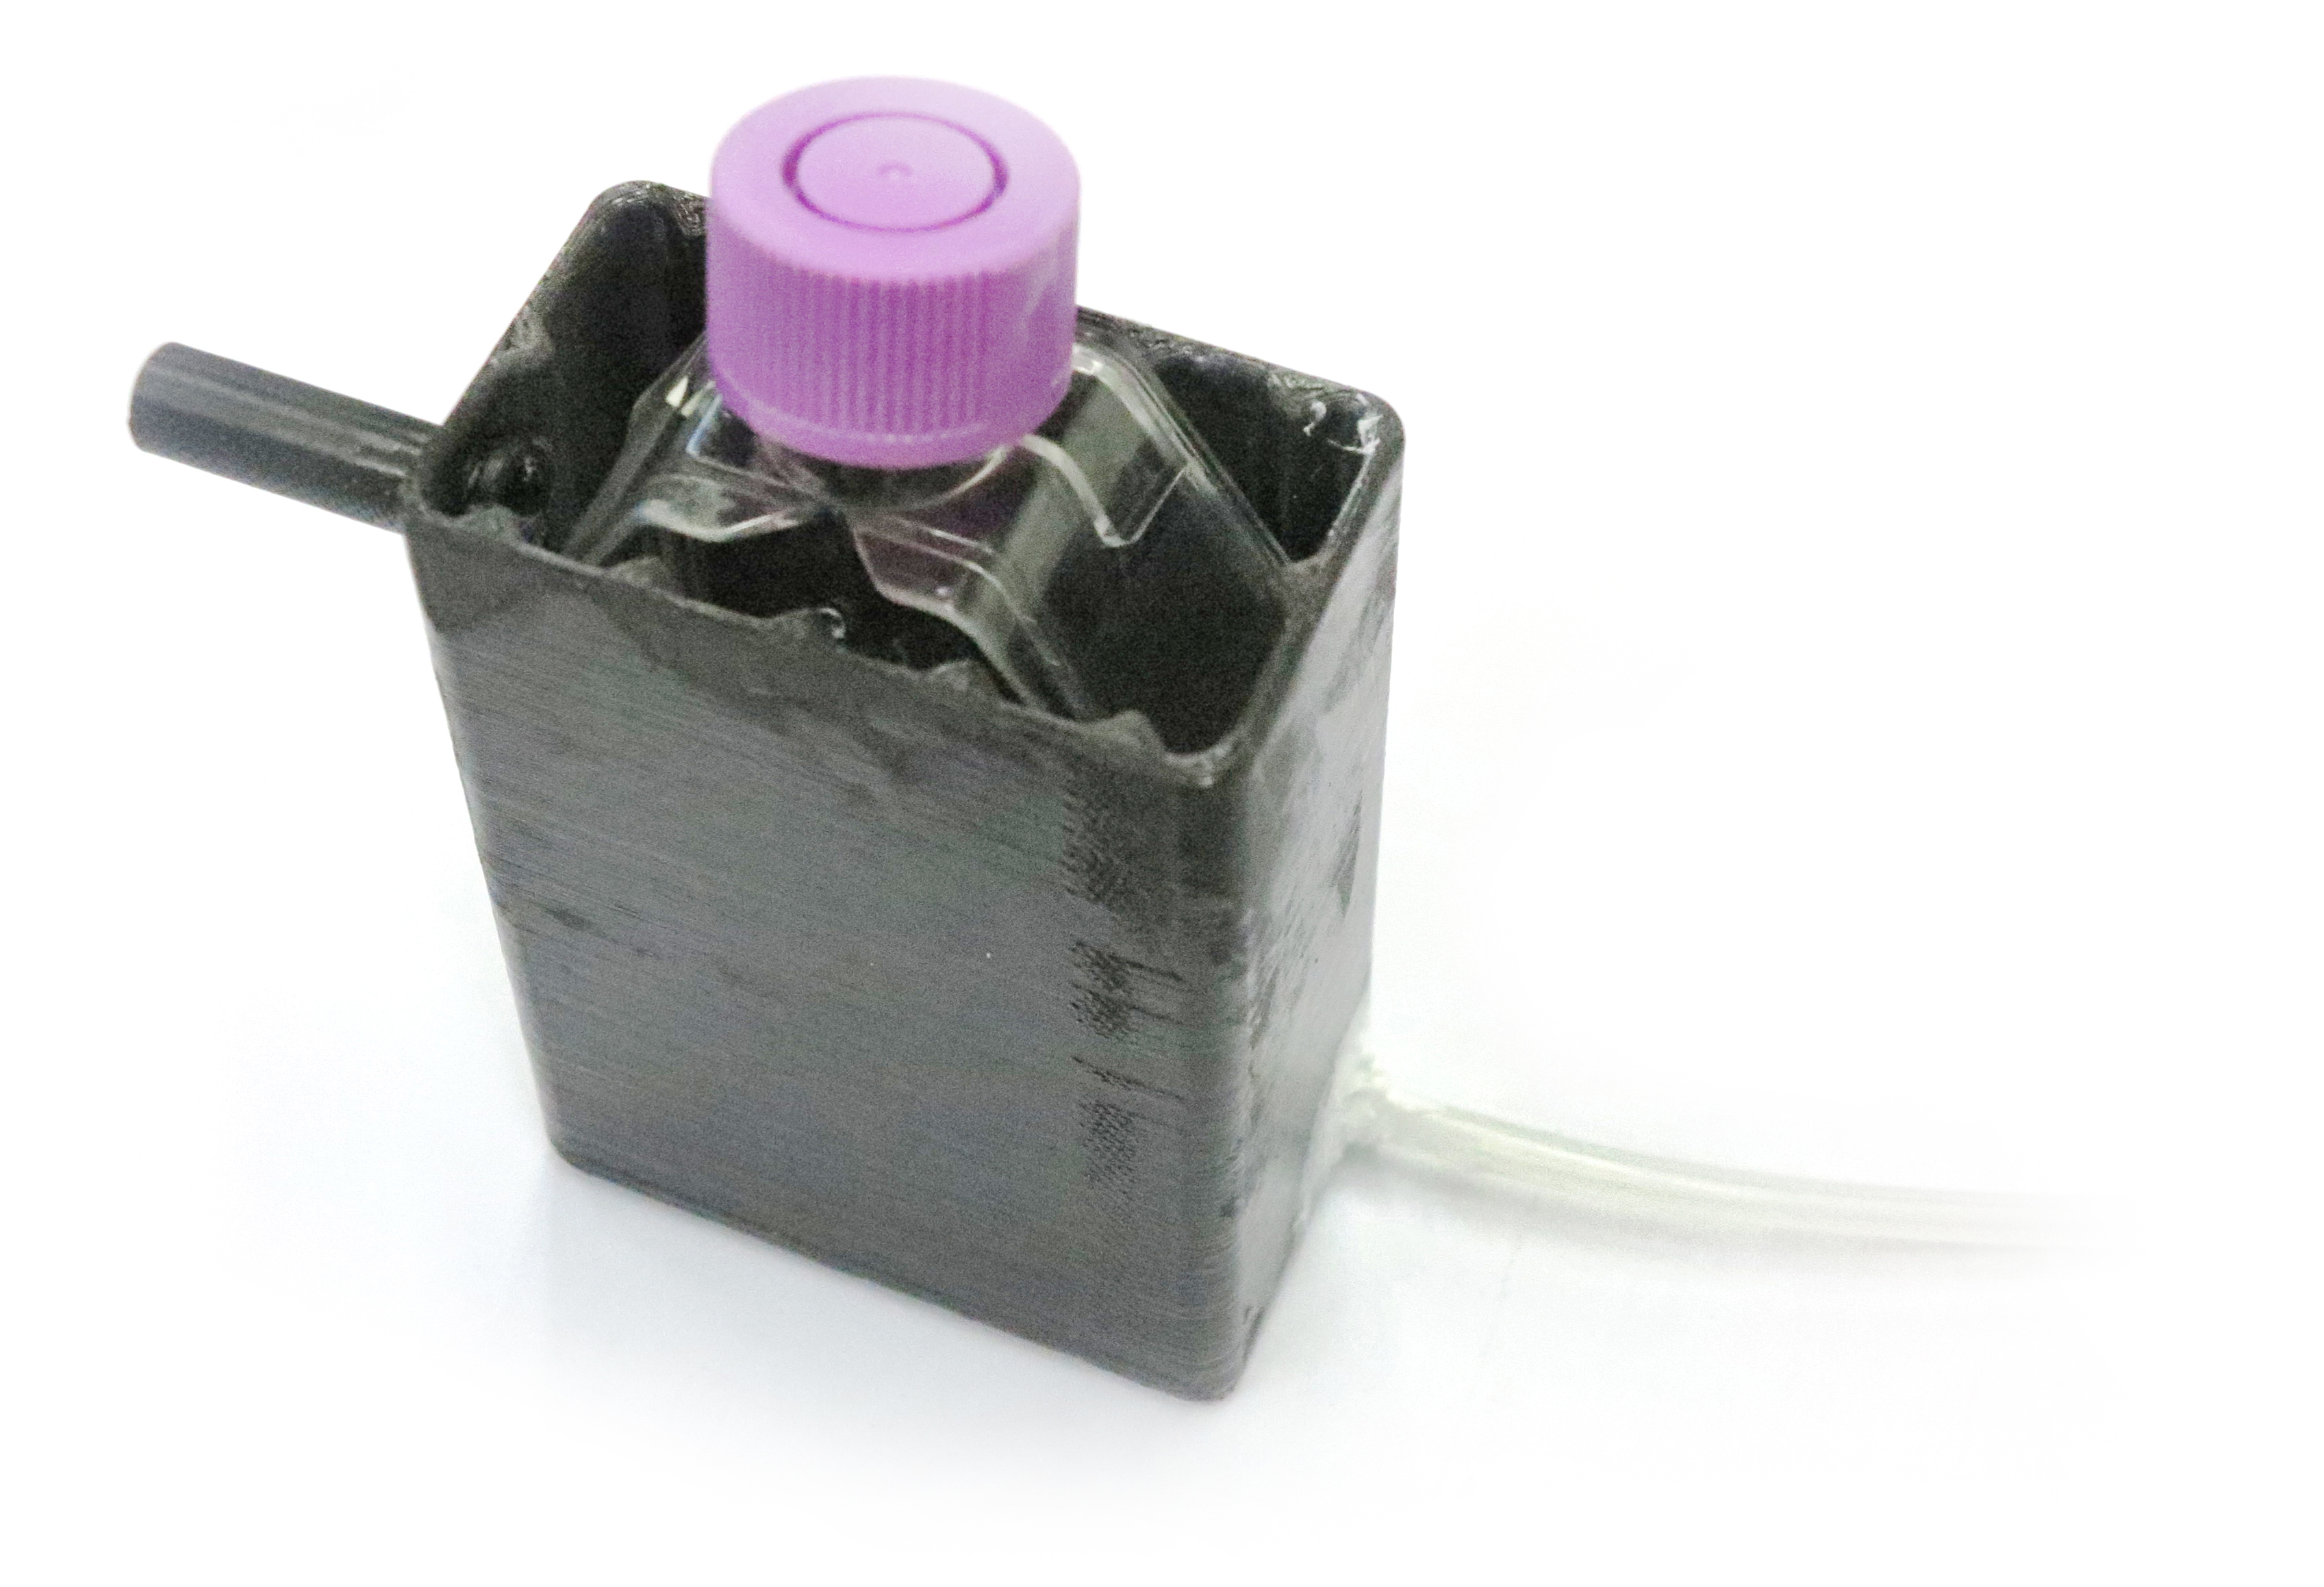
\includegraphics[width=0.45\textwidth]{image_heatExchanger.jpg}
 				\caption{Actual 3D Printed Heat Exchanger with an Algae Bottle}
 				\label{fig:actual_heatExchanger}
 			\end{center}
 		\end{figure}
 	
 	\section{Demonstration}
 		\begin{figure}[H]
 			\begin{center}
 				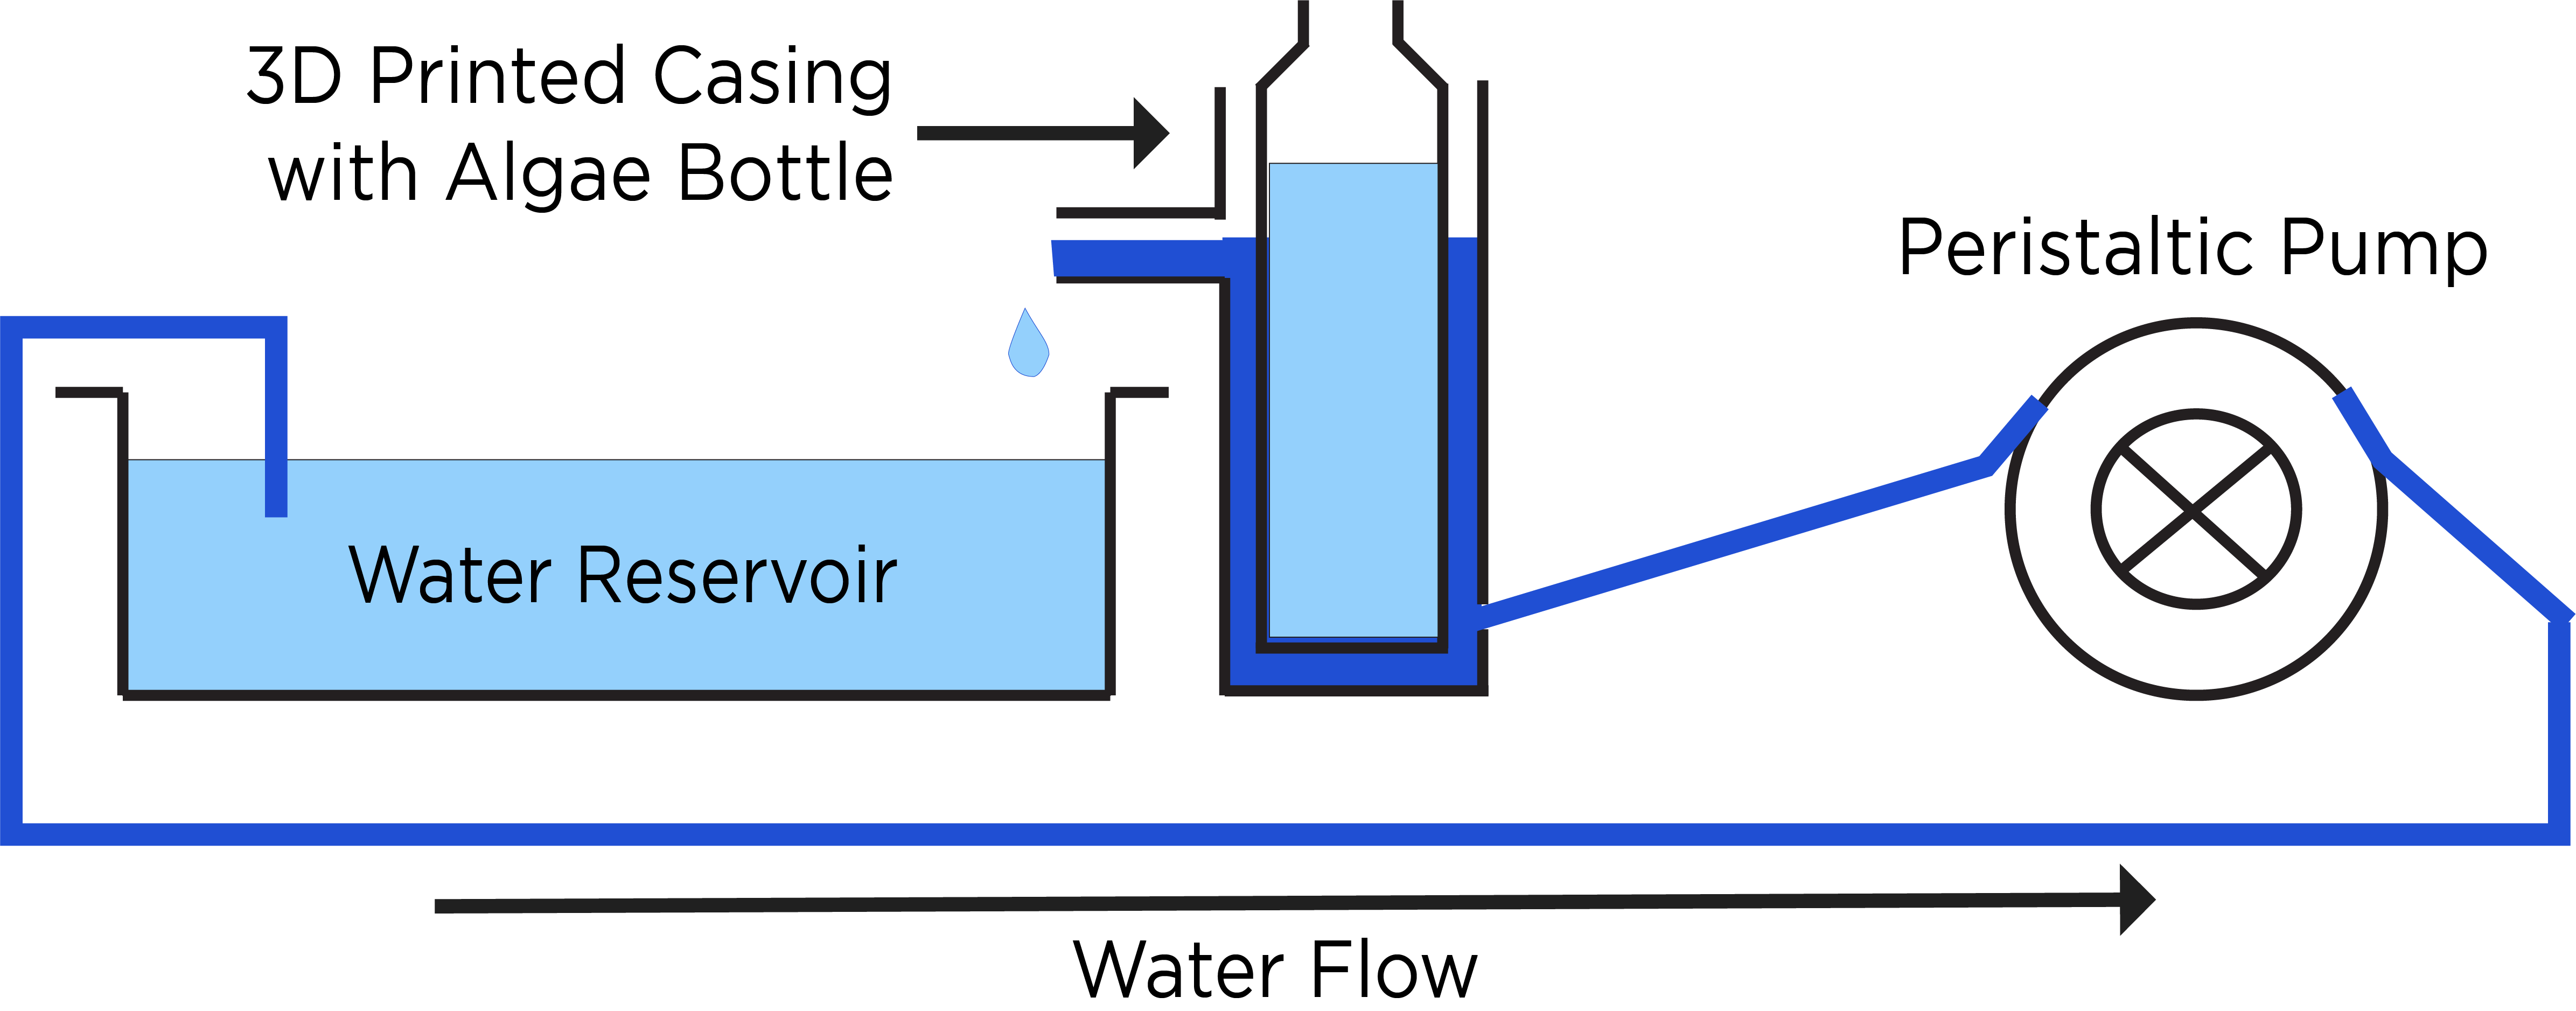
\includegraphics[width=0.4\textwidth]{demo_setup.png}
 				\caption{}
 				\label{fig:demo_setup}
 			\end{center}
 		\end{figure}
	 
	\section{Considering the Tubing as an Open System}
	If we consider the silicone tubing provided as an open system, the rate of change of energy in the control volume $\dot{E_{cv}}$ is given by:
	$$\dot{Q}_{cv} - \dot{W}_{cv} + \dot{m}_{i} \left( h_i + \frac{V_i}{2} + gz_i \right) + \dot{m}_{e} \left( h_e + \frac{V_e}{2} + gz_e \right)$$
	Assuming steady state, $\dot{m}_{i} = \dot{m}_{e} = \dot{m}$ and $\dot{E_{cv}} = 0$
	Thus the equation may be simplified to:
	$$\frac{dE_{cv}}{dt} = \dot{Q}_{cv} - \dot{W}_{cv} + \dot{m} \left( h_1 - h_2 \right)$$
	Expanding $\dot{Q}_{cv}$,
	$$\dot{Q}_{cv} = \dot{Q}_{exchanged} + \dot{Q}_{motor,water}$$
	
	\section{blah}
	\begin{enumerate}
		\def\labelenumi{\roman{enumi}.}
		\item The equation of control volume in the heat exchanger
		$$\frac{dE_{cv}}{dt} = \dot{Q}_{cv} - \dot{W}_{cv} + \dot{m}_{i} \left( h_i + \frac{V_i}{2} + gz_i \right) + \dot{m}_{e} \left( h_e + \frac{V_e}{2} + gz_e \right)$$ \\
		\textit{Assume steady state, so $\dot{m}_{i} = \dot{m}_{e} = \frac{dE_{cv}}{dt} = \dot{m}$ No change in potential and kinetic energy} \\
		\textit{Air is ideal gas.} \\
		$$\frac{dE_{cv}}{dt} = \dot{Q}_{cv} - \dot{W}_{cv} + \dot{m} \left( h_1 - h_2 \right)$$ \\
		\item The rate of heat entering control volume \\
		$$\dot{Q}_{cv} = \dot{Q}_{exchanged}$$ \\
		$$\dot{Q}_{cv} = m_a c_a \left( \frac{dT_a}{dt} \right) - \dot{Q}_{ambient}$$ \\
		$$\dot{Q}_{cv} = m_a c_a \left( \frac{dT_a}{dt} \right) - \lambda_{algaebottle} \left( T_a - T_{amb} \right)$$ \\
		\textit{By substituting value of $\lambda_{algaebottle} = 1.76$} \\
		$$\dot{Q}_{cv} = m_a c_a \left( \frac{dT_a}{dt} \right) - 1.76 \left( T_a - T_{amb} \right)$$ \\
		\item The equation of control volume in the heat exchanger \\
		\textit{From simplified $\frac{dE_{cv}}{dt}$ equation in the previous part} \\
		$$\frac{dE_{cv}}{dt} = \dot{Q}_{cv} - \dot{W}_{cv} + \dot{m} \left( h_1 - h_2 \right)$$ \\
		\item Express $\dot{W}_{cv}\ = f \left( T_a \right)$ assuming $\dot{W}_{cv}$ is a constant
		\textit{Assume that $\frac{dE_{cv}}{dt} = 0$} \\
		$$0 = m_a c_a \left( \frac{dT_a}{dt} \right) - \lambda_{algaebottle} \left( T_a - T_{amb} \right) - \dot{W}_{cv} + \dot{m} \lbrack c_w \left( T_i - T_e \right) \rbrack$$ \\
		$$\lambda_{algaebottle} \left( T_a - T_{amb} \right) + \dot{W}_{cv} - \dot{m} \lbrack c_w \left( T_i - T_e \right) \rbrack = m_a c_a \left( \frac{dT_a}{dt} \right)$$ \\
		$$\int 1 dt = \int \frac{m_a c_a}{\lambda_{algaebottle} \left( T_a - T_{amb} \right) + \dot{W}_{cv} - \dot{m} \lbrack c_w \left( T_i - T_e \right) \rbrack} dT_a$$ \\
		$$t+ c = \frac{m_a c_a}{\lambda_{algaebottle}} \ln(\lambda_{algaebottle} \left( T_a - T_{amb} \right) + \dot{W}_{cv} - \dot{m} \lbrack c_w \left( T_i - T_e \right) \rbrack)$$ \\
		$$\frac{\lambda_{algaebottle} \left( t + c \right)}{m_a c_a} = \ln(\lambda_{algaebottle} \left( T_a - T_{amb} \right) + \dot{W}_{cv} - \dot{m} \lbrack c_w \left( T_i - T_e \right) \rbrack)$$ \\
		$$e^{\frac{\lambda_{algaebottle} \left( t + c \right)}{m_a c_a}} = \lambda_{algaebottle} \left( T_a - T_{amb} \right) + \dot{W}_{cv} - \dot{m} \lbrack c_w \left( T_i - T_e \right) \rbrack$$ \\
		$$\dot{W}_{cv} = e^{\frac{\lambda_{algaebottle} \left( t + c \right)}{m_a c_a}} - \lambda_{algaebottle} \left( T_a - T_{amb} \right) + \dot{m} \lbrack c_w \left( T_i - T_e \right) \rbrack$$
	\end{enumerate}
	
	\section{Derivation}
	
	\bibliographystyle{IEEEtran}
	\bibliography{biblio}

\end{document}